% Text Mining and Search 2022/23

%-----------------------------------------------------------------
%	PACKAGES AND OTHER DOCUMENT CONFIGURATIONS
%-----------------------------------------------------------------

\documentclass[fleqn,10pt]{SelfArx} % Document font size and equations flushed left
\usepackage[english]{babel} % Specify a different language here - english by default
\usepackage{lipsum} % Required to insert dummy text. To be removed otherwise
\usepackage{float}

%-----------------------------------------------------------------
%	COLUMNS
%-----------------------------------------------------------------

\setlength{\columnsep}{0.75cm} % Distance between the two columns of text
\setlength{\fboxrule}{0.75pt} % Width of the border around the abstract

%-----------------------------------------------------------------
%	COLORS
%-----------------------------------------------------------------

\definecolor{color1}{RGB}{0,0,90} % Color of the article title and sections
\definecolor{color2}{RGB}{0,20,20} % Color of the boxes behind the abstract and headings

%-----------------------------------------------------------------
%	HYPERLINKS
%-----------------------------------------------------------------

\usepackage{hyperref} % Required for hyperlinks

\hypersetup{
	hidelinks,
	colorlinks,
	breaklinks=true,
	urlcolor=color2,
	citecolor=color1,
	linkcolor=color1,
	bookmarksopen=false,
	pdftitle={Title},
	pdfauthor={Author},
}

%-----------------------------------------------------------------
%	ARTICLE INFORMATION
%-----------------------------------------------------------------

\JournalInfo{Text Mining and Search} % Journal information
\Archive{UniMiB, 2022-23} % Additional notes (e.g. copyright, DOI, review/research article)

\PaperTitle{IMDB Reviews\\
\vspace{2mm}\large{Text Mining and Search}} % Article title

\Authors{Agazzi Ruben 844736, Cominetti Fabrizio 882737} % Authors
\affiliation{\textbf{University}: University of Milan-Bicocca} % Corresponding author

\Keywords{Text Mining --- Text Classification --- Text Clustering} % Keywords - if you don't want any simply remove all the text between the curly brackets
\newcommand{\keywordname}{Keywords} % Defines the keywords heading name

%-----------------------------------------------------------------
%	ABSTRACT
%-----------------------------------------------------------------

\Abstract{In this project, user reviews from the IMDB platform were analyzed through the use of text mining techniques. After carrying out an initial phase of text processing and text representation, the project continued with the classification of the reviews, through some text classification techniques - such as Support Vector Machines (SVM), Multilayer Perceptron (MLP), and Logistic Regression. Next, a text clustering phase was carried out through the use of two algorithms: DBSCAN and k-means.}

%-----------------------------------------------------------------

\usepackage{biblatex}
\addbibresource{ref.bib} %Import the bibliography file

%-----------------------------------------------------------------

\begin{document}

\maketitle % Output the title and abstract box

\tableofcontents % Output the contents section

\thispagestyle{empty} % Removes page numbering from the first page

%-----------------------------------------------------------------
%	ARTICLE CONTENTS
%-----------------------------------------------------------------

\section{Introduction}
The project aims to analyze the dataset "IMDB reviews" through text mining techniques, specifically through \textit{Text Classification} and \textit{Text Clustering}. The dataset contains a total amount of 50000 user-released reviews on the IMDB platform, divided in half between training and testing. The dataset is ideal for performing a binary sentiment classification task, the first objective of our analysis. Next, we decided to exploit text clustering techniques with the goal of identifying different clusters within the text.\\
Text Classification is the activity of predicting which data items belongs to a predefined finite set of classes. There are many types of classification, in our case it is \textit{Binary Classification}, where each item belongs to exactly one class in a set of two (positive or negative).\\
In addition, text classification may be performed according to several dimensions ('axes') orthogonal to each other. For example, by topic (the most frequent case), by sentiment - our case -, by language, by type, by author, by native language, by gender, and more.\\
Text clustering, on the other hand, is the task of grouping a set of unlabeled texts in such a way that texts in the same cluster are more similar to each other than to those in other clusters.

\section{Data}
As stated before, the dataset used contains a total of 50000 user reviews on the IMDB platform, a platform that describes itself in the following manner :"IMDb is the world's most popular and authoritative source for movie, TV and celebrity content. Find ratings and reviews for the newest movie and TV shows" \cite{IMDB}.\\
The dataset is also defined as a "Large Movie Review Dataset".\\
From an initial exploration of the data, we can observe that the dataset does not provide information about the date and reference film of the review, or any other indication, but contains only the text of the review and the extracted sentiment - positive or negative.\\
The data, initially divided into training and testing, but also between positive and negative sentiment, were merged, so that there would be a single dataset for the 25000 reviews to be used in the training phase and the 25000 reviews to be used in the testing phase.\\
Finally, the dataset contains precisely 12500 reviews labeled as positive and as many labeled as negative, both training and testing.

\section{Text Processing}
Having obtained the starting dataset, a series of \textit{Text Processing} operations were performed:
\begin{itemize}
	\item \textit{Remove Numbers}, all numbers within the text have been removed;
	\item \textit{Remove StopWords}, all words in the stopwords list have been removed;
	\item \textit{Remove Punctuation}, all punctuation has been removed;
	\item \textit{Remove Extra Space}, all extra spaces within the text have been removed;
	\item \textit{Tokenization}, the process of breaking down a text into units called tokens;
	\item \textit{Lower Case}, all words were converted to lower case;
	\item \textit{Lemmatization}, the process of grouping together the inflected forms of a word.
\end{itemize}

% esempio di frase prima e dopo processing

% I saw this movie at a drive-in in 1959. Until "Howard the Duck" I considered this the worst movie I had ever seen. This movie tried to combine all the genera in one; comedy, horror, teenage angst, and the hot rod that must have sired "My Mother, The Car." Maybe it deserves a second viewing to see if it is an accurate reflection of it's time.

% movie drivein howard duck considered worst movie movie combine genus comedy horror teenage angst hot rod sired mother car deserves viewing accurate reflection time

Below we can observe some basic statistics for the train and the test set. Precisely, the number of words in the corpus, and the average review length.

\begin{table}[ht]
\centering
\begin{tabular}{c c c }
	 & Train & Test  \\
	\hline
	Number of words & 24902 & 24798  \\
	Average review length & 685.01 & 668.02  \\
\end{tabular}
\caption{Statistics for train and test data}
\end{table}

In addition, we built two WordClouds, one for training set texts, the other for test set texts.

\begin{figure}[H]
\begin{center}
  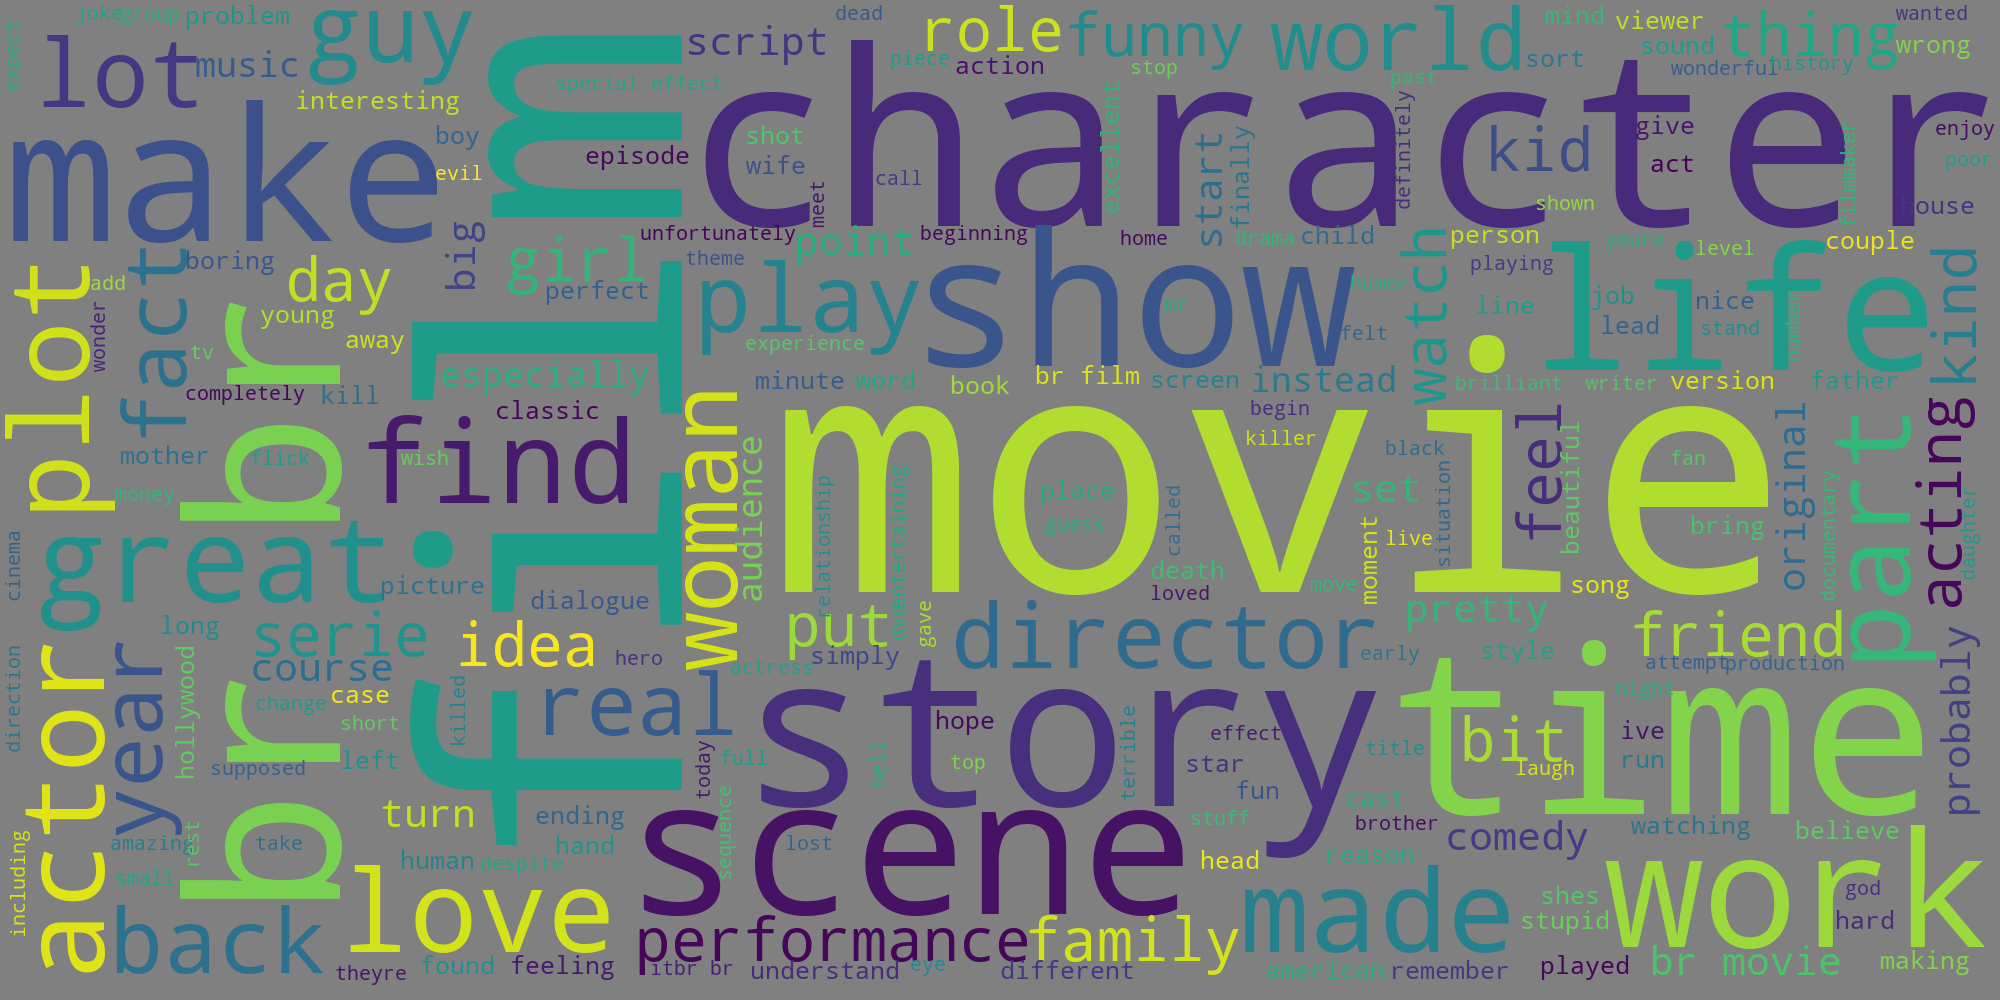
\includegraphics[scale=0.1]{./images/WordCloud_train.png}
\end{center}
  \caption{WordCloud - Training data}
\end{figure}

\begin{figure}[H]
\begin{center}
  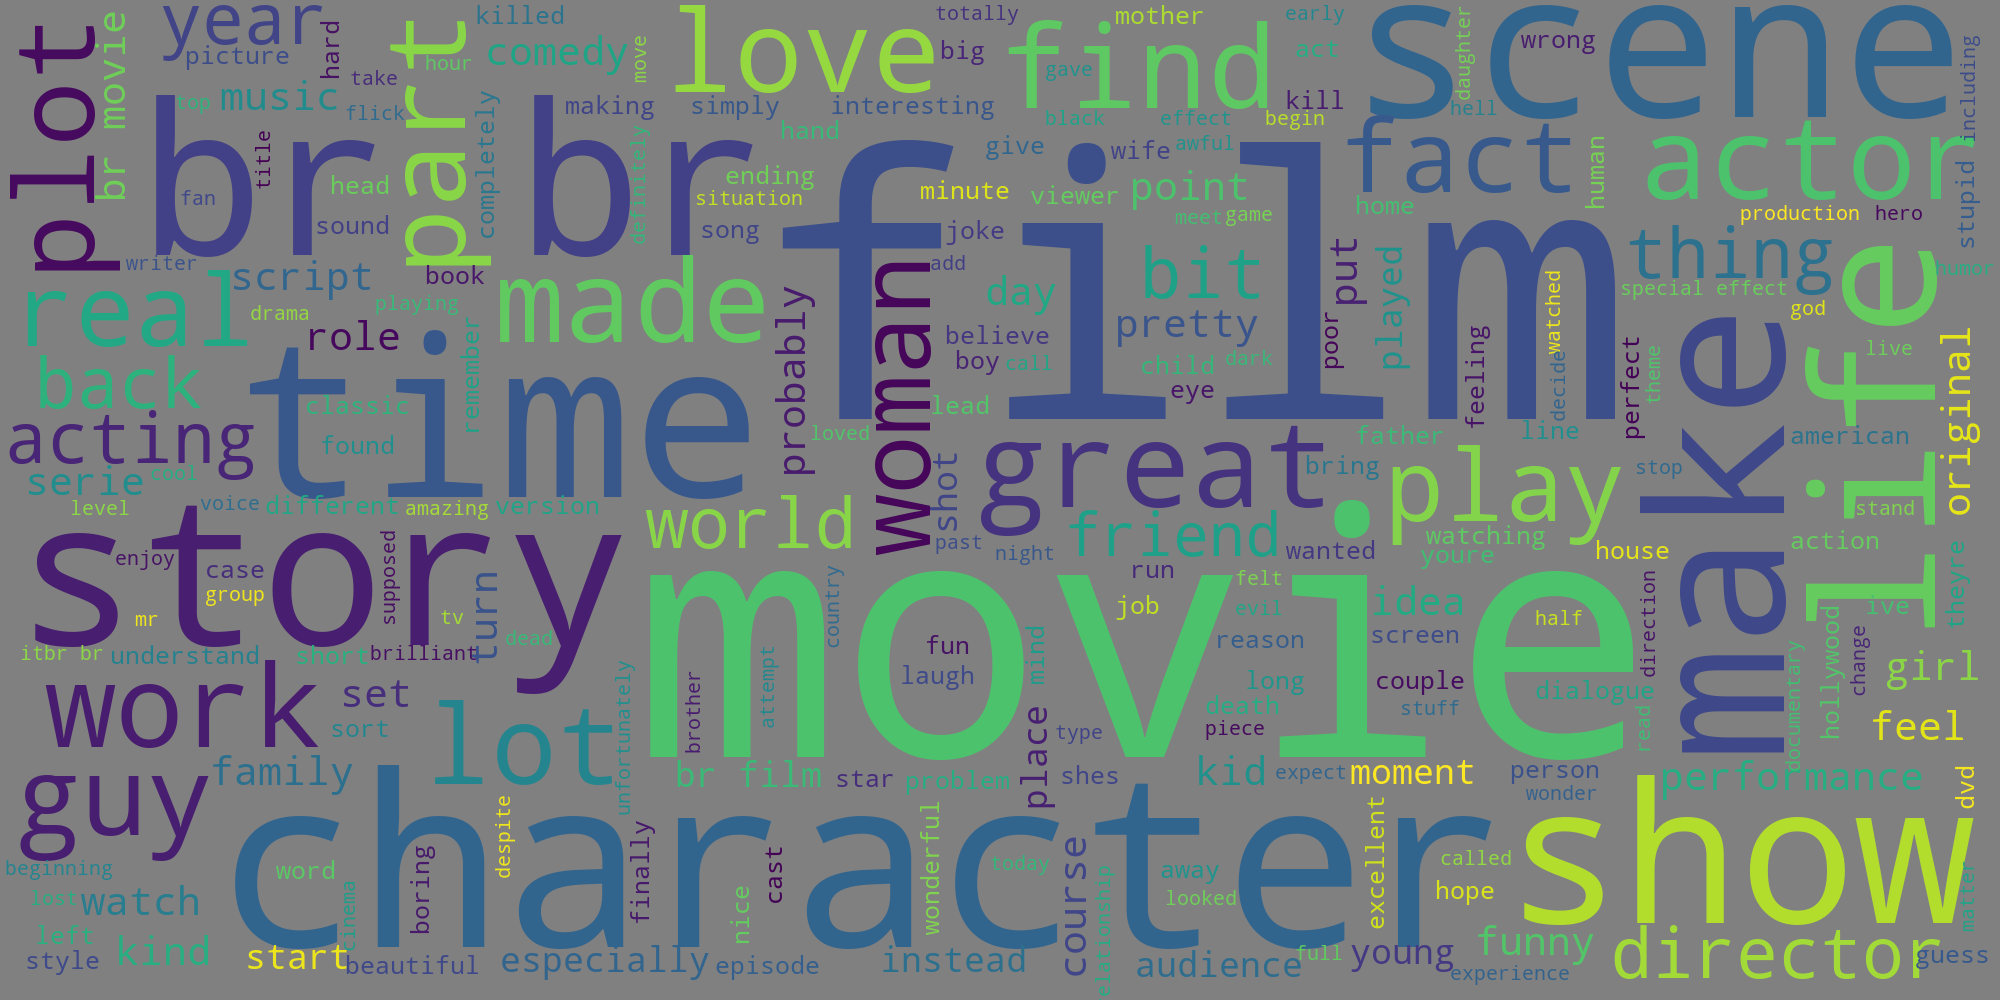
\includegraphics[scale=0.1]{./images/WordCloud_test.png}
\end{center}
  \caption{WordCloud - Test data}
\end{figure}

Once the corpus of texts had been properly processed, we moved on to the next stage of text representation.

\section{Text Representation}
Text Representation is the process to represent text with graphical methods. Considering the purposes of the project, the reviews were represented in structured form according to two methods: \textit{Bag of Words} and \textit{Tf-Idf}.\\
The Bag of Words representation identifies each document by a vector in which contains the number of occurrences of each word. This model doesn't consider grammar and order of words.\\
In the Tf-Idf representation, the number of occurrences of each word is weighted against the inverse of the word's presence in the corpus.\\
The weights, called \textit{Tf-Idf} weights, are the product of the two indices \textit{Tf} and \textit{Idf}:
\begin{center}
$w_{t,d} = \frac{tf_{t,d}}{max (tf_{t_i,d})} \times log(\frac{N}{df_t})$
\end{center}
Where the Term Frequency \textit{$tf_{t,d}$} represent the frequency of the term \textit{t} in the document \textit{d}, divided by the frequency of the most occurring word in the document to prevent bias towards longer documents; and the the Inverse Document Frequency \textit{$idf_t$} represents the inverse of the informativeness of the document for a term \textit{t}.\\
The two representations were implemented through two features of the sklearn package in python: CountVectorizer for Bag of Words, TfidfVectorizer for Tf-Idf. The range of n-grams chosen for both was 1-3, that is, Uni-grams Bi-grams, and Tri-grams. Tri-grams (three consecutive words) provide more context for text classification tasks than single words or bigrams (two consecutive words). By capturing the relationship between three words, tri-grams can better capture the meaning and context of text, improving the accuracy of text classification models.\\
Regarding the variable $'max\_features'$ corresponding to the maximum number of grams to be considered (the most frequent grams across the text), 10000 was chosen as the value.

\section{Text Classification}
Text Classification is the activity of predicting which data items belongs to a predefined finite set of classes. There are many types of classification, in our case it is \textit{Binary Classification}, where each item belongs to exactly one class in a set of two (positive or negative).\\
To pursue the goals of our project, we chose to use three classification algorithms, and for each of them we used the two types of text representation developed earlier.\\
The selected algorithms are as follows: Support Vector Machine (SVM), Multilayer Perceptron (MLP), and Linear Regression (LR).

\subsection{SVM}
Support vector machines (SVMs) are a set of supervised learning methods used for classification and other tasks \cite{SVM}. An SVM classifies data by finding the best hyperplane that separates all data points of one class from those of the other class. The best hyperplane for an SVM means the one with the largest margin between the two classes \cite{SVM2}. The advantages of support vector machines are its effectiveness in high dimensional spaces, its effectiveness in cases where the number of dimensions is greater than the number of samples, its memory efficiency, and its versatility. On the other side, the disadvantages of support vector machines include the fact that if the number of features is much greater than the number of samples, avoiding over-fitting in choosing Kernel functions and regularization term is crucial, and also SVMs do not directly provide probability estimates.\\
In our case, we used the LinearSVC package built on scikit-learn.

\begin{figure}[H]
\begin{center}
  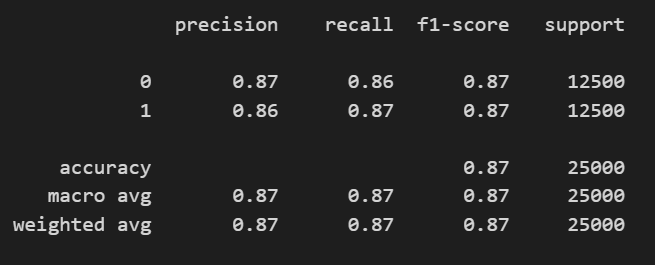
\includegraphics[scale=0.6]{./images/SVM_BoW.png}
\end{center}
  \caption{Classification report - SVM with Bag-of-Words}
\end{figure}

\begin{figure}[H]
\begin{center}
  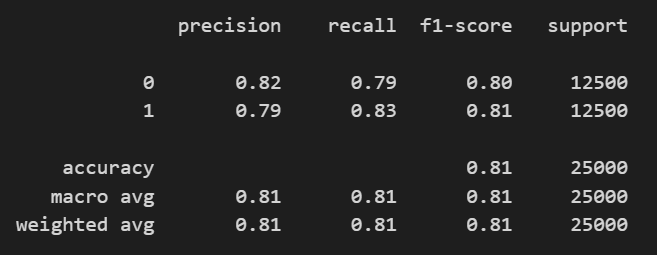
\includegraphics[scale=0.6]{./images/SVM_TFIDF.png}
\end{center}
  \caption{Classification report - SVM with Tf-Idf}
\end{figure}

As we can observe above, accuracy is better with Bag-of-Words, with a value of 0.87.

\subsection{Multilayer Perceptron}
Multilayer perceptron (MLP) is a supplement of feed forward neural network. It consists of three types of layers: the input layer, output layer and hidden layer \cite{MLP}.\\
The input layer receives the input signal to be processed. The required task such as prediction and classification is performed by the output layer. An arbitrary number of hidden layers that are placed in between the input and output layer are the true computational engine of the MLP.\\
In our case we exploited the potential of Keras. Keras is an open source library for machine learning and neural networks in Python.

\begin{figure}[H]
\begin{center}
  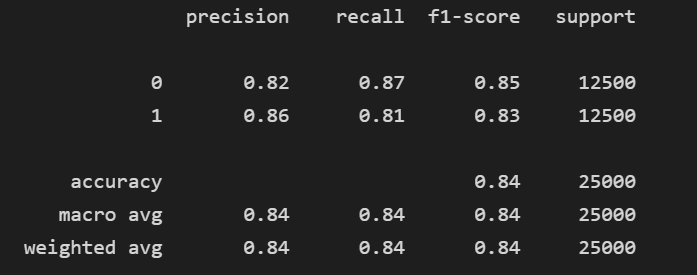
\includegraphics[scale=0.6]{./images/MLP_BoW.png}
\end{center}
  \caption{Classification report - MLP with Bag-of-Words}
\end{figure}

\begin{figure}[H]
\begin{center}
  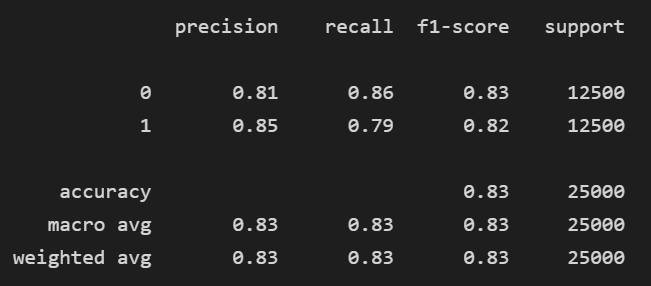
\includegraphics[scale=0.6]{./images/MLP_TFIDF.png}
\end{center}
  \caption{Classification report - MLP with Tf-Idf}
\end{figure}

As we can observe above, accuracy is the same for the two models, with a value of 0.83.

\subsection{Logistic Regression}
Logistic Regression is a statistical approach and a Machine Learning algorithm that is used for classification problems and is based on the concept of probability \cite{LR}. It is widely used when the classification problem at hand is binary. Logistics regression uses the sigmoid function to return the probability of a label.\\
In our case, we used the LogisticRegression package built on scikit-learn.

\begin{figure}[H]
\begin{center}
  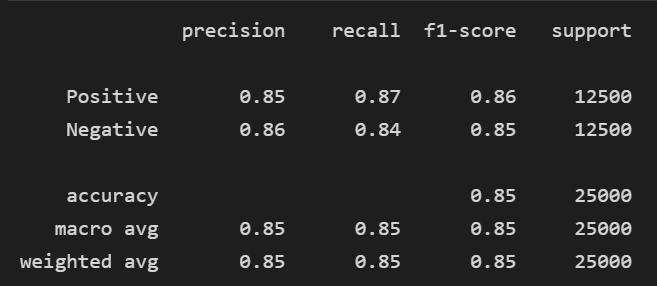
\includegraphics[scale=0.6]{./images/LR_BoW.png}
\end{center}
  \caption{Classification report - LR with Bag-of-Words}
\end{figure}

\begin{figure}[H]
\begin{center}
  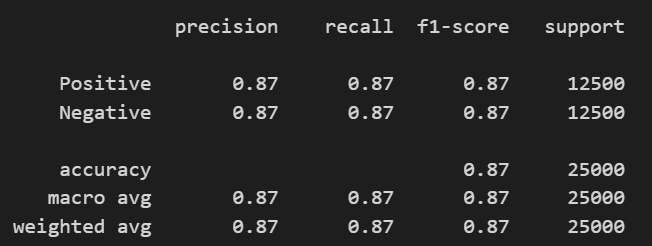
\includegraphics[scale=0.6]{./images/LR_TFIDF.png}
\end{center}
  \caption{Classification report - LR with Tf-Idf}
\end{figure}

As we can observe above, in this case instead the accuracy is better with Tf-Idf, with a value of 0.87.

\subsection{Evaluation}
The highest accuracy value is obtained with the Logistic Regression algorithm with Tf-Idf weights, and with Support Vector Machine with Bag-of-Words.

\section{Text Clustering}
Text clustering is the task of grouping a set of unlabeled texts in such a way that texts in the same cluster are more similar to each other than to those in other clusters. Text clustering algorithms process text and determine if natural clusters (groups) exist in the data \cite{textClustering}.\\
The big idea is that documents can be represented numerically as vectors of features. The similarity in text can be compared by measuring the distance between these feature vectors. Objects that are near each other should belong to the same cluster. Objects that are far from each other should belong to different clusters.\\
Clustering can be divided into two groups:
\begin{itemize}
	\item \textit{Hard Clustering}: each item is assigned to only one cluster;
	\item \textit{Soft Clustering}: an item can belong to multiple clusters.
\end{itemize}

There are also different types of clustering structure:
\begin{itemize}
	\item Partitional, a division of the set of data objects into non-overlapping subsets (clusters) such that each data object is in exactly one subset vs Hierarchical, sub-clusters organized as a tree;
	\item Exclusive, each data object is assigned to a single cluster vs Overlapping, data can be assigned in more than one cluster;
	\item Complete, every data is assigned to a cluster vs Partial, where every data is not necessary assigned to a cluster.
\end{itemize}

The goals of text clustering for a reviews dataset are various and can include segmentation, dividing the reviews into meaningful groups based on some criteria (like sentiment), to identify patterns and trends within the data; summarization, to create a compact representation of the reviews by summarizing topics, sentiments, or keywords; and, in general, to better understand the data and users' opinions and preferences. But also, to enable a more efficient information retrieval, and to reduce the number of reviews by grouping similar reviews together.\\
% The mapping from textual data to real-valued vectors is called feature extraction. One of the simplest techniques to numerically represent text is Bag of Words (BOW). In BOW, we make a list of unique words in the text corpus called vocabulary. Then we can represent each sentence or document as a vector, with each word represented as 1 for presence and 0 for absence. Another representation is to count the number of times each word appears in a document. The most popular approach is using the Term Frequency-Inverse Document Frequency (TF-IDF) technique.
We used two different clustering algorithms to identify different clusters from the total number of reviews in the dataset. Before we began, however, we performed dimensionality reduction of the total dataset - training plus testing - using Singular Value Decomposition (SVD).\\
SVD can be useful for text clustering as it provides a computationally efficient and effective way to reduce the dimensionality of large and sparse document-term matrices. SVD can transform the high-dimensional document-term matrix into a low-dimensional representation, which can then be used to cluster the documents based on their similarity. The reduced dimensionality representation of documents obtained through SVD it's used as input to the clustering algorithms.\\
Also, for the clustering phase we used the Tf-Idf vectorizer with 10000 as $'max\_features'$, and we considered only Uni-grams and Bi-grams for reasons of computational efficiency. Using only uni-grams and bi-grams, in fact, can provide a good balance between accuracy and computational efficiency in text clustering tasks.\\
For each model, we visualized the clusters and calculated the Silhouette coefficient. Then, for each cluster identified by the models, we developed wordclouds.

\subsection{DBSCAN}
DBSCAN, or \textit{Density-Based Spatial Clustering of Applications with Noise}, is an unsupervised machine learning algorithm used for text clustering.  It works by grouping together text documents that are similar to each other based on their density of word occurrences. It can be used for clustering data points based on density, by grouping together areas with many samples. This makes it especially useful for performing clustering under noisy conditions.\\
Density-based means that it will zoom into areas that have great density, or in other words a large amount of samples closely together. Spatial clustering means that it performs clustering by performing actions in the feature space. In other words, whereas some clustering techniques work by sending messages between points, DBSCAN performs distance measures in the space to identify which samples belong to each other. Clustering speaks for itself, and applications with noise means that the technique can be used with noisy datasets \cite{DBSCAN}.\\
The algorithm starts by selecting a random document as a "seed" and then finds all the other documents that are close to it, where "close" is defined by a user-specified distance metric (e.g. cosine similarity). If a sufficient number of documents are found to be close to the seed, they are all grouped together into a cluster. The algorithm then repeats this process for each cluster, until all the documents have been assigned to a cluster. The key advantage of DBSCAN is that it can identify clusters of arbitrary shapes, which is useful in text clustering where clusters may not be spherical.

\begin{figure}[H]
\begin{center}
  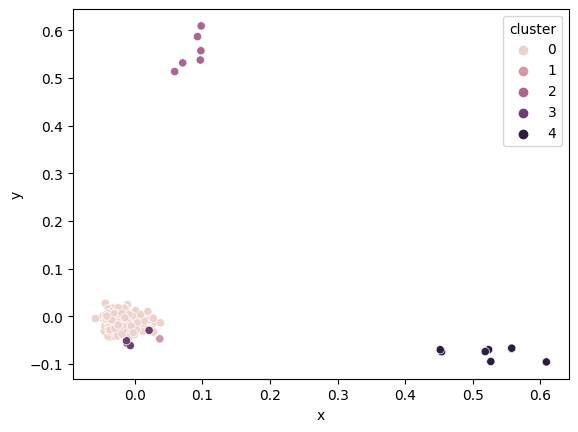
\includegraphics[scale=0.5]{./images/dbscan.png}
\end{center}
  \caption{DBSCAN - Clustering}
\end{figure}

\subsection{K-means}
K-means clustering is a type of unsupervised learning method. The goal of this algorithm is to find groups in the data, whereas the number of groups is represented by the variable k.\\
The k-means algorithms take input data and a predefined number of clusters as input. This method does not guarantee convergence to the global solution, and its results may depend upon the initial cluster center.\\
The k-means algorithm is defined as follows:
\begin{enumerate}
	\item Select k objects as centroids;
	\item Form k clusters and assign each document to the closest centroid;
	\item Compute the centroid for each cluster;
	\item Go to 1. until centroids do not change.
\end{enumerate}

In our case, we chose 4 as the number of clusters to be specified to the algorithm.

\begin{figure}[H]
\begin{center}
  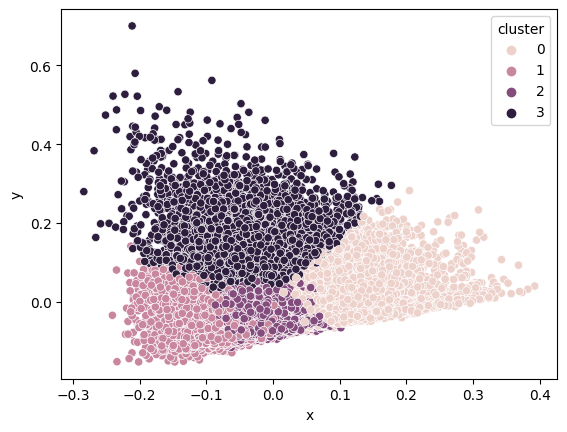
\includegraphics[scale=0.5]{./images/k-means.png}
\end{center}
  \caption{k-means - Clustering}
\end{figure}

\subsection{Evaluation}
A good clustering algorithm will produce high quality clusters in which the intra-class (that is, intra-cluster) similarity is high, and the inter-class similarity is low.\\
The most important Internal Evaluation index is the Silhouette Coefficient, that measures how well an observation is clustered and estimates the average distance between clusters.\\
The Silhouette Coefficient is calculated using the mean intra-cluster distance $a(i)$ and the mean nearest cluster distance $b(i)$ for each sample $i$:\\

\begin{center}
$S(i) = \frac{b(i) - a(i)}{max(a(i), b(i))}$
\end{center}

$S(i)$ will lie between [$ -1,1 $]:
\begin{itemize}
	\item If the Silhouette value is close to 1, the sample is well clustered and already assigned to a very appropriate cluster;
	\item If Silhouette value is about to 0, the sample could be assigned to another cluster closest to it and the sample lies equally far away from both the clusters. That means it indicates overlapping clusters;
	\item If Silhouette value is close to -1, the sample is misclassified and is merely placed somewhere in between the clusters.
\end{itemize}

The following are the value of the Silhouette coefficient for the selected algorithms:

\begin{table}[ht]
\centering
\begin{tabular}{c c c }
	 & DBSCAN & K-means  \\
	\hline
	Silhouette Index & 0.391 & 0.017  \\
\end{tabular}
\caption{Silhouette Coefficient}
\end{table}

As we can observe from the above table, the Silhouette value for the DBSCAN algorithm is higher than for the K-means algorithm.\\
We can state that the clusters obtained with DBSCAN are more appropriate and the sample is better clustered than with K-means.

Below, we can observe the wordclouds for each cluster identified by the DBSCAN algorithm:

\begin{figure}[H]
\begin{center}
  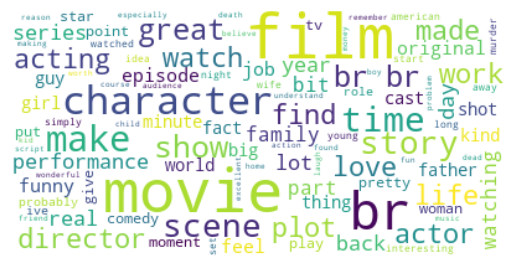
\includegraphics[scale=0.5]{./images/dbscan_wordcloud1.png}
\end{center}
\end{figure}

\begin{figure}[H]
\begin{center}
  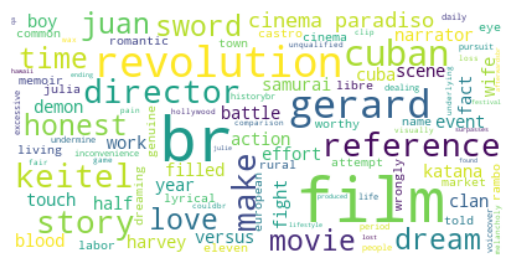
\includegraphics[scale=0.5]{./images/dbscan_wordcloud2.png}
\end{center}
\end{figure}

\begin{figure}[H]
\begin{center}
  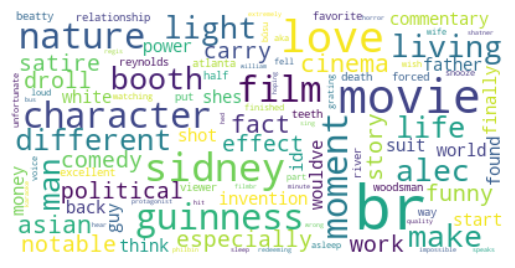
\includegraphics[scale=0.5]{./images/dbscan_wordcloud3.png}
\end{center}
\end{figure}

\begin{figure}[H]
\begin{center}
  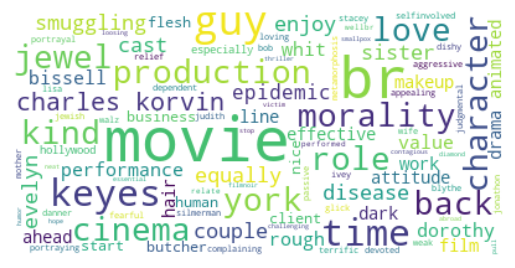
\includegraphics[scale=0.5]{./images/dbscan_wordcloud4.png}
\end{center}
\end{figure}

\begin{figure}[H]
\begin{center}
  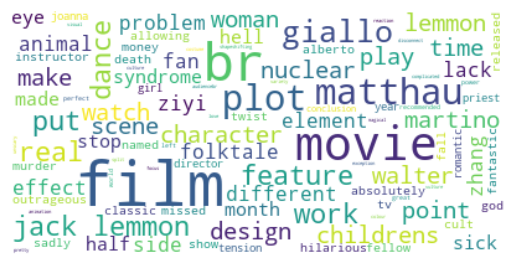
\includegraphics[scale=0.5]{./images/dbscan_wordcloud5.png}
\end{center}
\end{figure}

Below, instead, we can observe the wordclouds for each cluster identified by the K-means algorithm:

\begin{figure}[H]
\begin{center}
  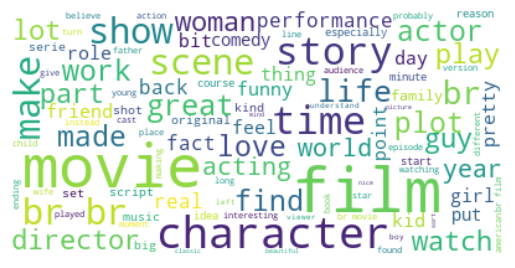
\includegraphics[scale=0.5]{./images/kmeans_wordcloud1.png}
\end{center}
\end{figure}

\begin{figure}[H]
\begin{center}
  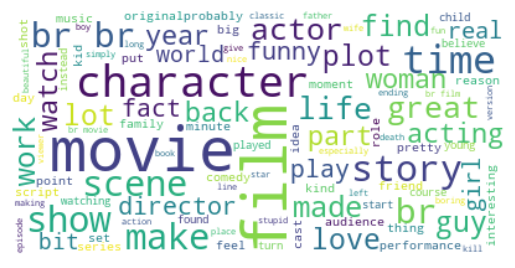
\includegraphics[scale=0.5]{./images/kmeans_wordcloud2.png}
\end{center}
\end{figure}

\begin{figure}[H]
\begin{center}
  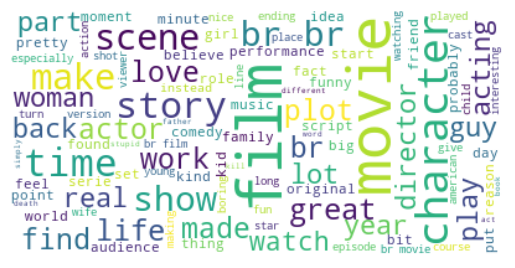
\includegraphics[scale=0.5]{./images/kmeans_wordcloud3.png}
\end{center}
\end{figure}

\begin{figure}[H]
\begin{center}
  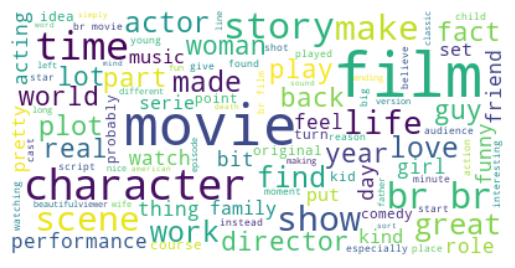
\includegraphics[scale=0.5]{./images/kmeans_wordcloud4.png}
\end{center}
\end{figure}

\section{Summary}
In conclusion, we can be satisfied with what we obtained from the text classification phase, with all three algorithms achieving a good accuracy value. In addition, the Silhouette coefficient values obtained by the text clustering algorithms are not equally satisfactory. Possible future developments could include different algorithms and different text representation techniques.

%%%%%%%%%%%%%%%%%%%%%%%%%%%%%%%%%%%%%%%%%%%%%%%%%%%%%%%%%%%%%%%%%

\nocite{*}
\printbibliography

\end{document}